\chptr{Gravitazione}
\marginpar{\minitoc}

\section{Gravità e forze fondamentali}
Conosciamo bene la seconda legge della dinamica $\vecsymb{F} = m\vecsymb{a}$.
Sappiamo che il termine $\vecsymb{F}$ rappresenta l'azione di un agente esterno,
chiamato forza, che può avere natura diversa a seconda del sistema studiato.
Pertanto, possiamo esprimere
la sua intensità in forme a volte diverse, sia essa il peso, l'attrito, la
forza elastica e così via. Tuttavia tutte queste forze, per quanto sappiamo al
giorno d'oggi, sono riconducibili a quattro interazioni fondamentali che si
manifestano nella materia (dalla più forte alla più debole):
\begin{itemize}
    \item \textit{Forza forte}: la più forte tra tutte. Tiene insieme i nuclei
    degli atomi.

    \item \textit{Forza elettromagnetica}: accoppia le cariche elettriche e
    le correnti.

    \item \textit{Forza debole}: si manifesta in fenomeni di decadimento nucleare.
    
    \item \textit{Forza gravitazionale}: la più debole tra tutte.
\end{itemize}
Lo stato attuale della fisica suggerisce che molte di queste forze possano essere
unificate, ovvero esse non sono altro che la manifestazione, in nature differenti,
della stessa forza fondamentale.
Sorprendentemente, è stata la forza più debole ad essere studiata per prima.
La legge fondamentale venne formulata da Newton nel seguente modo:

\vspace{8pt}
\begin{tcolorbox}[colback = yellow!30, colframe = yellow!30!black, title = {Legge di gravitazione universale}]
    \begin{align}
        \vecsymb{F}_{\text{G}, 1\to 2} = -G\frac{m_{\text{G},1}m_{\text{G},2}}{r^2_{1,2}}\hat{r}_{1,2}\label{gravity}
    \end{align}    
\end{tcolorbox}
\vspace{5pt}

\begin{marginfigure}
    \centering
    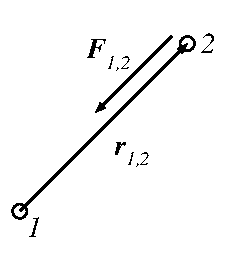
\includegraphics[width = \marginparwidth]{gravity.pdf}
    \caption{Illustrazione dell'applicazione della legge di Newton.
    Anche se non viene mostrata, il corpo 2 esercita la stessa
    forza, ma opposta in verso, sul corpo 1, in accordo con la
    terza legge della dinamica.}
    \label{gravitescionalfors}
\end{marginfigure}

\noindent Che esprime il vettore della forza gravitazionale che un corpo 1 esercita su un
altro corpo 2. Come mostrato in figura \ref{gravitescionalfors}, il vettore giace sulla congiungente tra i due corpi (considerati come
punti materiali), separati da una distanza $r_{1,2}$ e dotati di una certa
\textit{massa gravitazionale} $m_G$. Il segno negativo, accompagnato dalla
\textit{costante di gravitazione universale}, indica che la forza gravitazionale è
sempre attrattiva.

\section{Il principio di equivalenza}
Soffermiamoci a chiarire alcuni concetti. Innanzitutto, vogliamo esprimere la legge
\ref{gravity} in maniera più generica.

\begin{align}
    \vecsymb{F} = c\frac{p_1p_2}{r^2}\hat{r} \label{template}
\end{align}

\noindent Sorprendentemente, questa forma verrà proposta da Coulomb per esprimere
l'interazione tra due cariche elettriche, secondo la legge (in moduli)

\[ F_E = k\frac{|q_1||q_2|}{r^2} \]

\noindent Diventa naturale pensare che la \ref{template} possa rappresentare una
sorta di ``template'' con il quale esprimere quantitativamente l'interazione tra due
oggetti dotati di una certa qualità o proprietà intrinseca $p$, che consente agli oggetti in
questione di partecipare nell'interazione. Nel caso delle cariche elettriche,
essa sarà, per l'appunto, una carica elettrica. Per quanto riguarda la gravità,
questa qualità è la massa gravitazionale. Ci si può chiedere se stiamo parlando
della stessa massa della seconda legge di Newton. In realtà, esse sono ben diverse:
\begin{itemize}
    \item La massa inerziale $m_I$ esprime la capacità di un corpo di opporsi all'azione
    di agenti esterni e, di conseguenza, al cambiamento del proprio stato di moto.
    In breve, essa misura l'inerzia del corpo.

    \item La massa gravitazionale $m_G$ esprime la capacità di un corpo di partecipare,
    contribuire ed essere soggetto all'interazione gravitazionale in presenza di
    un altro corpo dotato di massa gravitazionale.
\end{itemize}
Seppur sottile, la differenza tra queste quantità è
comunque diversa (un oggetto ``massivo'' è difficile da spostare; un oggetto ``massiccio''
interagisce maggiormente con un altro oggetto). La parola ``carica'' sarebbe più intuitiva per spiegare la differenza
e viene infatti utilizzata per le interazioni elettriche: più ``carico'' di una certa
proprietà dell'interazione, più ``intensa'' l'interazione stessa. Nella pratica ci
riferiamo sempre alla stessa massa (i kilogrammi), ma nulla impedisce di pensare che le masse di
uno stesso corpo siano effettivamente quantità distinte.

Consideriamo un corpo in prossimità della superficie terrestre. Possiamo approssimare
la Terra ad una sfera uniforme e supporre che la forza gravitazionale corpo-Terra
giaccia sulla congiungente tra il centro del pianeta e il corpo (puntiforme). Il
corpo si trova ad una certa altezza $h$ e conosciamo inoltre il raggio della Terra
$R_T$. Il corpò sarà soggetto alla forza gravitazionale della Terra; uniamo le
equazioni di Newton (consideriamo i moduli):
\[ F = m_\text{I,C}a \qquad F = G\frac{m_\text{G,C}M_\text{G,T}}{(R_{T} + h)^2} \]
Supponiamo che $R_T \gg h$. Dunque la distanza Terra-corpo può essere approssimata:
\[ r_\text{T,C} = R_T + h = R_T\left(1 + \frac{h}{R_T}\right) \]
\[ r_\text{T,C}^2 \simeq R_T^2\left( 1 + 2\frac{h}{R_T} \right) \]
\[ \frac{1}{r_\text{T,C}^2} \simeq \frac{1}{R_T^2}\left( 1 - 2\frac{h}{R_T} \right) \]

\noindent Da cui concludiamo che possiamo trascurare $h$. Dunque, sapendo che
$a = g$,

\[ m_\text{I,C}g = G\frac{m_\text{G,C}M_\text{G,T}}{R_{T}^2} \]

\noindent Isoliamo $g$

\[ g = \frac{m_\text{G,C}}{m_\text{I,C}}G\frac{M_\text{G,T}}{R_{T}^2} \]

\noindent Se assumessimo che le masse inerziale e gravitazionale di uno stesso corpo
sono diverse, l'accelerazione $g$ non sarebbe la stessa per tutti gli oggetti. Tuttavia,
non è ancora stata trovata evidenza della differenza quantitativa (apprezzabile, in
quanto misure sperimentali) tra le due proprietà. L'osservazione galileiana stessa
sulla caduta libera, ovvero che tutti i corpi cadono con la stessa accelerazione,
indica che

\begin{align}
    m_I = m_G\label{equivalence}
\end{align}

\noindent che rappresenta il principio di equivalenza tra massa inerziale e massa
gravitazionale. Possiamo affermare ciò perché,
fisttata la massa della Terra e il suo raggio,
il rapporto $m_I/m_G$ deve essere costante
affinché $g$ sia uguale per tutti i corpi di massa distinta.

\section{Approfondimenti}
Forse il campo della fisica più affascinante è
l'astrofisica. Citiamo solo alcuni approfondimenti infinitesimi rispetto
all'immensità della fisica astronomica\footnote{Così ampia per via della
sua storia millenaria, al contrario della meccanica descritta in queste
pagine}.

\subsection{Energia potenziale gravitazionale}
Si usa spesso calcolare l'energia potenziale di un oggetto vicino alla superficie
terrestre, ad un'altitudine $h$, con la seguente legge:

\[ mgh \]

\noindent Tuttavia sappiamo che $g$ non è costante al variare della quota e su grandi
distanze questa legge non è più una buona approssimazione. Calcoliamo dunque la differenza
di energia potenziale tra la superficie terrestre e una certa quota $h$ da essa alla luce
della legge di Newton.

\[ \Delta\mathcal{U} = -W = -\int_{R}^{R + h}-G\frac{mM}{s^2}\,ds = GmM\int_{R}^{R+h}\frac{ds}{s^2} = GmM\left[ -\frac{1}{s} \right]_{R}^{R+h} =  \]
\[ = -GmM\left( \frac{1}{R + h} - \frac{1}{R} \right) \]

\noindent Notiamo che $\Delta\mathcal{U} > 0$, dunque allontanando un oggetto di massa
$m$ dalla superficie terrestre, esso guadagna una certa energia potenziale. Più in generale,
se poniamo un punto di riferimento $X$ arbitrario dal quale calcolare la (differenza di)
energia potenziale verso un punto $P$, otteniamo la seguente espressione:

\[ \mathcal{U}(P) = -GmM\left(\frac{1}{r_P} - \frac{1}{r_X}\right) \]

\noindent Per convenienza è utile porre $r_X = +\infty$, ovvero ad una distanza infinita da
$M$, ottenendo dunque

\[ \mathcal{U} = -\frac{GmM}{r} \]

\noindent L'energia meccanica di un corpo è dunque

\[ E = E_K + \mathcal{U} = \frac{1}{2}mv^2 -\frac{GmM}{r} \]

\noindent Ovviamente supponiamo che tutte queste leggi valgano per punti materiali.
In un caso reale, per esempio per il calcolo dell'energia potenziale gravitazionale
in prossimità della Terra, quando si ``sprofonda'' nel corpo che genera il campo
gravitazionale, l'estensione di tale corpo modifica l'andamento dell'energia potenziale.

\subsection{Eratostene e Cavendish}
Per giungere alla conclusione mostrata nell'equazione \ref{equivalence},
sono necessari due dati molto importanti: Il raggio della Terra e la
costante $G$. Il primo fu misurato già ai tempi di Eratostene. Il secondo
rimase incognito per quasi 100 anni dopo la formulazione della legge
\ref{gravity} da parte di Newton.

Nel 1798 il fisico inglese Henry Cavendish compì un esperimento con
strumentazioni abbastanza sensibili da poter stimare il valore di $G$,
un dato estremamente piccolo (ordine $10^{-11}$!). Nel suo esperimento,
Cavendish utilizzà una bilancia di torsione. Due masse $m$ sono fissate
a un'asta appesa ad un filo (la massa dell'asta è trascurabile).
Accando alle due masse sospeso sono poste due grandi masse $M > m$ ferme.
Ciascuna massa $m$ viene attratta, a causa della forza di gravità,
verso la massa $M$ vicina, quindi l'asta che sostiene le masse sospese
ruota e torce il filo. È possibile misurare l'angolo di torsione del
filo riflettendo un raggio di luce su una superficie riflettente
solidale con il filo. Se è nota la forza necessaria per torcere il
filo di un dato angolo (questo è possibile se il filo è stato tarato
con esperimenti precedenti), la misura dell'angolo di torsione fornisce
la maisura dell'intensità della forza di gravità. Conoscendo le masse
$m$ e $M$ e la distanza tra i loro centri, possiamo usare la legge
di Newton per per ricavare $G$.
Cavendish ottenne un valore $G = 6.754 \cdot 10^{-11} Nm^2/kg^2$,
in accordo con il valore oggi accettato di $6.67 \cdot 10^{-11} Nm^2/kg^2$.

Avendo a disposizione il valore di $G$, fu quindi possibile determinare
anche la massa della Terra $M_T$:

\[ M_T = \frac{gR_T^2}{G} \]

\subsection{Gravitazione universale}
Secondo la legge di Newton, tutti gli oggetti nell'universo si attraggono l'un l'altro
attraverso l'interazione gravitazionale. è in questo senso che la legge viene detta
``universale''.

%\subsubsection{Modelli astronomici}

\subsubsection{La terza legge di Keplero}
Ovviamente la legge di Newton ha grande importanza in campo astronomico (anche
se espressa in forme assai più complesse) ed è stata la conferma di una legge scoperta
sperimentalmente tempo addietro da Keplero, appunto la \textit{terza legge di Keplero}:

\[ T \propto r^\frac{3}{2} \]

\noindent Secondo tale legge, il periodo $T$ di rivoluzione di un pianeta attorno al Sole
è proporzionale alla distanza media $r$ del pianeta dal Sole elevata a $3/2$. Dunque esiste
una costante $k$ tale che $T = kr^\frac{3}{2}$. In realtà
questa legge vale per tutti i sistemi astronomici (solari e non) simili al nostro, ma
gli studi di Keplero si basavano sugli attenti dati raccolti dal maestro Tycho Brahe
sui moti orbitali dei corpi celesti appartenenti al sistema solare.

Per dimostrare la terza legge per via teorica, è necessario supporre che il pianeta
in rivoluzione intorno al Sole viaggia secondo un moto circolare uniforme\footnote{Anche se in realtà
l'orbita è ellittica, la distanza media tra pianeta e Sole è la stessa durante una rivoluzione e dunque il
moto è approssimabile a quello circolare.}, del quale conosciamo bene le relazioni che legano periodo, velocità
angolare, velocità tangenziale e accelerazione centripeta: $T = 2\pi/\omega$, $v = \omega r$ e
$a_c = v^2/r$.
Sapendo poi che la forza di gravità tra un pianeta e il Sole è proprio la forza
centripeta del moto orbitale, possiamo effettuare i seguenti calcoli unendo tutte
le leggi scoperte fino ad ora:

\[ T = \frac{2\pi}{\omega} = \frac{2\pi}{v}r = \frac{2\pi}{\sqrt{a_c r}}r = \frac{2\pi}{\sqrt{\frac{GM}{r}}}r = \left(\frac{2\pi}{\sqrt{GM}}\right)r^\frac{3}{2} \]

\noindent Non solo abbiamo dimostrato la terza legge, ma abbiamo pure individuato la
costante di proporizonalità $k$.

\subsubsection*{Sistemi binari}
Dedichiamo questa sezione ad un classico problema di gravitazione piuttosto complesso,
ma altrettanto interessante, presente peraltro in natura nonostante il classico
modello copernicano al quale siamo abituati.

In sistemi non simili a quello solare vale ancora la legge di Newton. Consideriamo
per esempio un sistema di stelle binarie, ovvero stelle con una differenza di massa
non trascurabile rispetto alla distanza del centro di massa del sistema dal centro
di massa di una delle due stelle. In tale caso, le stelle orbiteranno attorno al
loro centro di massa, situato in qualche punto dello spazio intermedio sulla loro
congiungente. Anche nel sistema solare la Terra e il Sole ruotano attorno al centro
di massa totale, che tuttavia si trova ben al di sotto della superficie del Sole,
il che permette di ridurre la trattazione del problema ad una rivoluzione della
Terra attorno al Sole.